\documentclass{article}
\usepackage{graphicx}
\usepackage[utf8]{inputenc}

\usepackage{tikz}
% load circuits library
\usetikzlibrary{
  circuits.logic,
  circuits.logic.US,
  positioning
}
\title{SIT111}
\author{Niroshinie Fernando}
\date{March 2021}

\begin{document}

\section{Week1}
\subsection{Topic3}
\subsubsection{Boolean Operations – Gate Representation, slide no 7}
\paragraph{AND gate:}
The AND gate symbol is given in Figure \ref{fig:andgate}.

\begin{figure}[h]
\centering
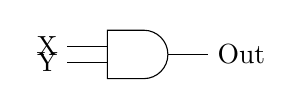
\begin{tikzpicture}[circuit logic US]
 \node[and gate] (and) {};
    \draw (and.input 1)--++(180:.5cm) node[left] (x) {X};
    \draw (and.input 2)--++(180:.5cm) node[left] (y) {Y};
    \draw (and.output)--++(360:.5cm) node[right] (o) {Out};

\end{tikzpicture}
\caption{The AND Gate Symbol} 
\label{fig:andgate}
\end{figure}

This can also be written as:
\begin{itemize}
\item X AND Y
\item X*Y
\end{itemize}

\paragraph{OR gate}
The OR gate symbol is given in Figure \ref{fig:orgate}.

\begin{figure}[h]
\centering
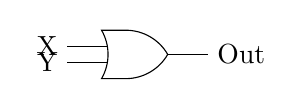
\begin{tikzpicture}[circuit logic US]
 \node[or gate] (or) {};
    \draw (or.input 1)--++(180:.5cm) node[left] (x) {X};
    \draw (or.input 2)--++(180:.5cm) node[left] (y) {Y};
    \draw (or.output)--++(360:.5cm) node[right] (o) {Out};

\end{tikzpicture}
\caption{The AND Gate Symbol} 
\label{fig:orgate}
\end{figure}

This can also be written as:
\begin{itemize}
\item X OR Y
\item X+Y
\end{itemize}

\paragraph{NOT gate}
The NOT gate symbol is given in Figure \ref{fig:notgate}.

\begin{figure}[h]
\centering
\begin{tikzpicture}[circuit logic US]
 \node[not gate] (not) {};
    \draw (not.input)--(180:.5cm) node[left] (x) {X};
    \draw (or.output)--++(360:.5cm) node[right] (o) {Out};

%         \draw
% (0,4) node[not port, scale=.5](mynotA){}
% (mynotA.in) node[left=1](a) {A}
% (a) -- (mynotA.in)
\end{tikzpicture}
\caption{The NOT Gate Symbol} 
\label{fig:notgate}
\end{figure}

This can also be written as:
\begin{itemize}
\item NOT X
\item $\overline{X}$
\end{itemize}


\maketitle

\section{Introduction}

\end{document}
